\documentclass[11pt]{article} 
\usepackage{geometry} 
\geometry{letterpaper} 
\usepackage{graphicx} 
\usepackage{amssymb} 
\usepackage{amsmath} 
\usepackage{epstopdf} 
\usepackage{hyperref} 
\usepackage{natbib} 
\DeclareGraphicsRule{.tif}{png}{.png}{`convert #1 `dirname #1`/`basename #1 .tif`.png} 
\graphicspath{
{/Users/Andy/Cruises_Research/OceanMixingGroup/cruises/ctd_chipod/IO8/}
{/Users/Andy/Cruises_Research/OceanMixingGroup/cruises/ctd_chipod/IO8/figures/}
{/Users/Andy/Cruises_Research/OceanMixingGroup/cruises/ctd_chipod/IO8/figures/XC/}
{/Users/Andy/Cruises_Research/OceanMixingGroup/cruises/ctd_chipod/IO8/figures/proc/SN1013/}
{/Users/Andy/Cruises_Research/OceanMixingGroup/cruises/ctd_chipod/IO8/figures/proc/SN2020/}
{/Users/Andy/Cruises_Research/OceanMixingGroup/cruises/ctd_chipod/IO8/figures/proc/SN2014/}
{/Users/Andy/Cruises_Research/OceanMixingGroup/cruises/ctd_chipod/IO8/figures/proc/SN2009/}
{/Users/Andy/Cruises_Research/OceanMixingGroup/cruises/ctd_chipod/IO8/figures/proc/SN2004/}
{/Users/Andy/Cruises_Research/OceanMixingGroup/cruises/ctd_chipod/IO8/figures/proc/SN2003/}
{/Users/Andy/Cruises_Research/OceanMixingGroup/cruises/ctd_chipod/IO8/figures/proc/SN2002/}
{/Users/Andy/Cruises_Research/OceanMixingGroup/cruises/ctd_chipod/IO8/figures/proc/SN2001/}
} 

\title{IO8 CTD-Chipod Notes} 
\author{Andy Pickering} 
\begin{document} 
\maketitle 
\tableofcontents 
\newpage 

%~~~~~~~~~~~~~~~~~~~~~~~~~~
 \section{About} 

Notes on processing and analysis of CTD-chipod data collected during IO8 cruise.. 

\begin{figure}[htbp] 
\includegraphics[width=38pc]{IO8_kml_map.jpg} 
\caption{Map of CTD cast locations during cruise IO8.} 
\label{map} 
\end{figure} 



\section{Data and Processing} 

Data paths are set w/ :  
\begin{itemize} 
\item \verb+Load_chipod_paths_IO8.m+ 
\end{itemize} 

Chipod deployment info is given in  
\begin{itemize} 
\item \verb+Chipod_Deploy_Info_IO8+ 
\end{itemize} 

$s\subsection{CTD} 

Raw (hex) CTD data are processed with: 
\begin{itemize} 
\item \verb+Process_CTD_hex_IO8.m+ 
\end{itemize} 

$s\subsection{Chipod} 

\begin{table}[htdp] 
\caption{Summary of Chipod deployment .} 
\begin{center} 
\begin{tabular}{|c|c|c|c|} 
\hline 
\end{tabular} 
\end{center} 
\label{default} 
\end{table}Raw chipod files are plotted with  
\begin{itemize} 
\item \verb+PlotChipodDataRaw_IO8.m+ 
\end{itemize} 
to check for obvious issues/malfunctions with any of the instruments; these plots are saved in erb+/Figures/chipodraw/+.  
Based on a quick look at these: 
\begin{itemize} 
\item 
\end{itemize} 

Files with obviously bad or missing data (based on above raw plots) are noted in erb+bad_file_list_XXXX.m+ and, which will prevent them from being loaded in the processing. 

Processing scripts are: 
\begin{itemize} 
\item \verb+MakeCasts_CTDchipod_IO8.m+ 
\item \verb+DoChiCalc_IO8.m+ 
\end{itemize} 

$s\subsection{Further processing and analysis} 

\begin{itemize} 
\item Data from all casts are combined into a single structure w/ erb+MakeCombinedStruct_IO8.m+ 
\item  
\end{itemize} 

\newpage 

%~~~~~~~~~~~~~~~~~~~~~~~~~~
 \section{Processing Notes} 

\begin{itemize} 
\item Table 
ef{chidepinfo} gives the info for $\item Table 
ef{procsum} gives a summary of the processing from MakeCasts. 
\end{itemize} 

% make and insert table 1 

% make and insert table 2 

% continue... 

$s\subsubsection{Time Offsets} 

\begin{figure}[htbp] 

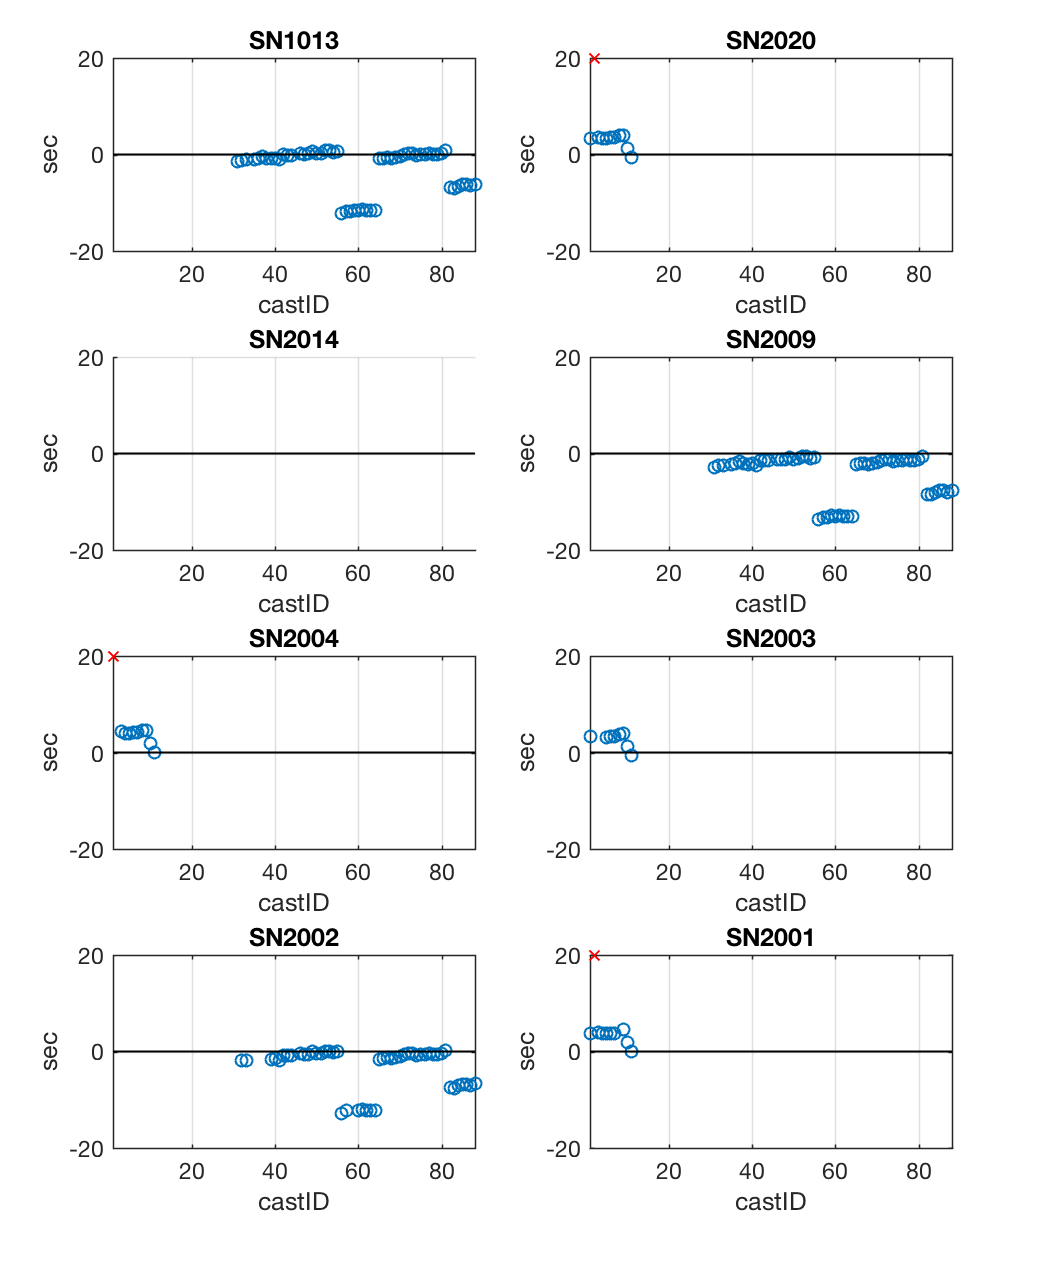
\includegraphics[scale=1]{IO8_timeoffsets_all.png} 
\caption{Time-offsets for all $\chi$pods, found by aligning with CTD data.} 
\label{toffs} 
\end{figure} 

\newpage 

%~~~~~~~~~~~~~~~~~~~~~~~~~~
 \section{Example Raw Chipod Data for 1 cast} 

\begin{figure}[htbp] 
\includegraphics[scale=0.7]{SN1013_001_Fig1_RawChipodTS.png} 
\caption{Raw chipod data from SN1013for a CTD cast.} 
\label{SN1013_1} 
\end{figure} 

\begin{figure}[htbp] 
\includegraphics[scale=0.7]{SN2020_001_Fig1_RawChipodTS.png} 
\caption{Raw chipod data from SN2020for a CTD cast.} 
\label{SN2020_1} 
\end{figure} 

\begin{figure}[htbp] 
\includegraphics[scale=0.7]{SN2014_001_Fig1_RawChipodTS.png} 
\caption{Raw chipod data from SN2014for a CTD cast.} 
\label{SN2014_1} 
\end{figure} 

\begin{figure}[htbp] 
\includegraphics[scale=0.7]{SN2009_001_Fig1_RawChipodTS.png} 
\caption{Raw chipod data from SN2009for a CTD cast.} 
\label{SN2009_1} 
\end{figure} 

\begin{figure}[htbp] 
\includegraphics[scale=0.7]{SN2004_001_Fig1_RawChipodTS.png} 
\caption{Raw chipod data from SN2004for a CTD cast.} 
\label{SN2004_1} 
\end{figure} 

\begin{figure}[htbp] 
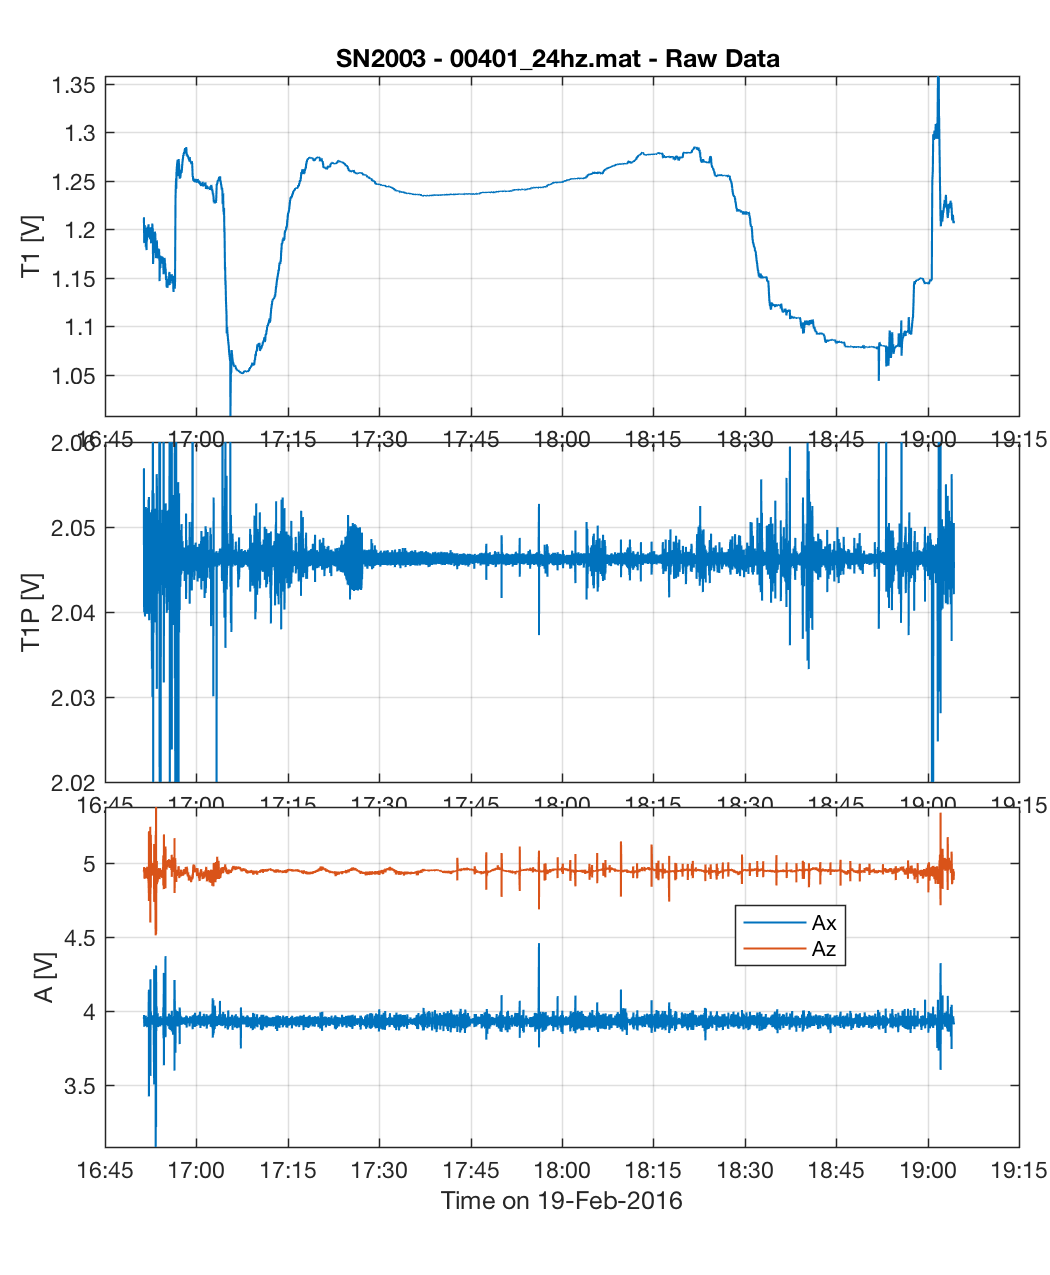
\includegraphics[scale=0.7]{SN2003_Cast_00401_Fig1_RawChipodTS.png} 
\caption{Raw chipod data from SN2003for a CTD cast.} 
\label{SN2003_1} 
\end{figure} 

\begin{figure}[htbp] 
\includegraphics[scale=0.7]{SN2002_001_Fig1_RawChipodTS.png} 
\caption{Raw chipod data from SN2002for a CTD cast.} 
\label{SN2002_1} 
\end{figure} 

\begin{figure}[htbp] 
\includegraphics[scale=0.7]{SN2001_001_Fig1_RawChipodTS.png} 
\caption{Raw chipod data from SN2001for a CTD cast.} 
\label{SN2001_1} 
\end{figure} 

\newpage 



\section{Results} 

\clearpage 

$s\subsubsection{CTD Data } 
\begin{figure}[htbp] 
\includegraphics[scale=0.7]{IO8_ctd_t_s.png} 
\caption{Plot of temperature and salinity from CTD downcasts on all casts.} 
\label{} 
\end{figure} 

\clearpage 

$s\subsubsection{Data from each individual Chipod} 

\begin{figure}[htbp] 
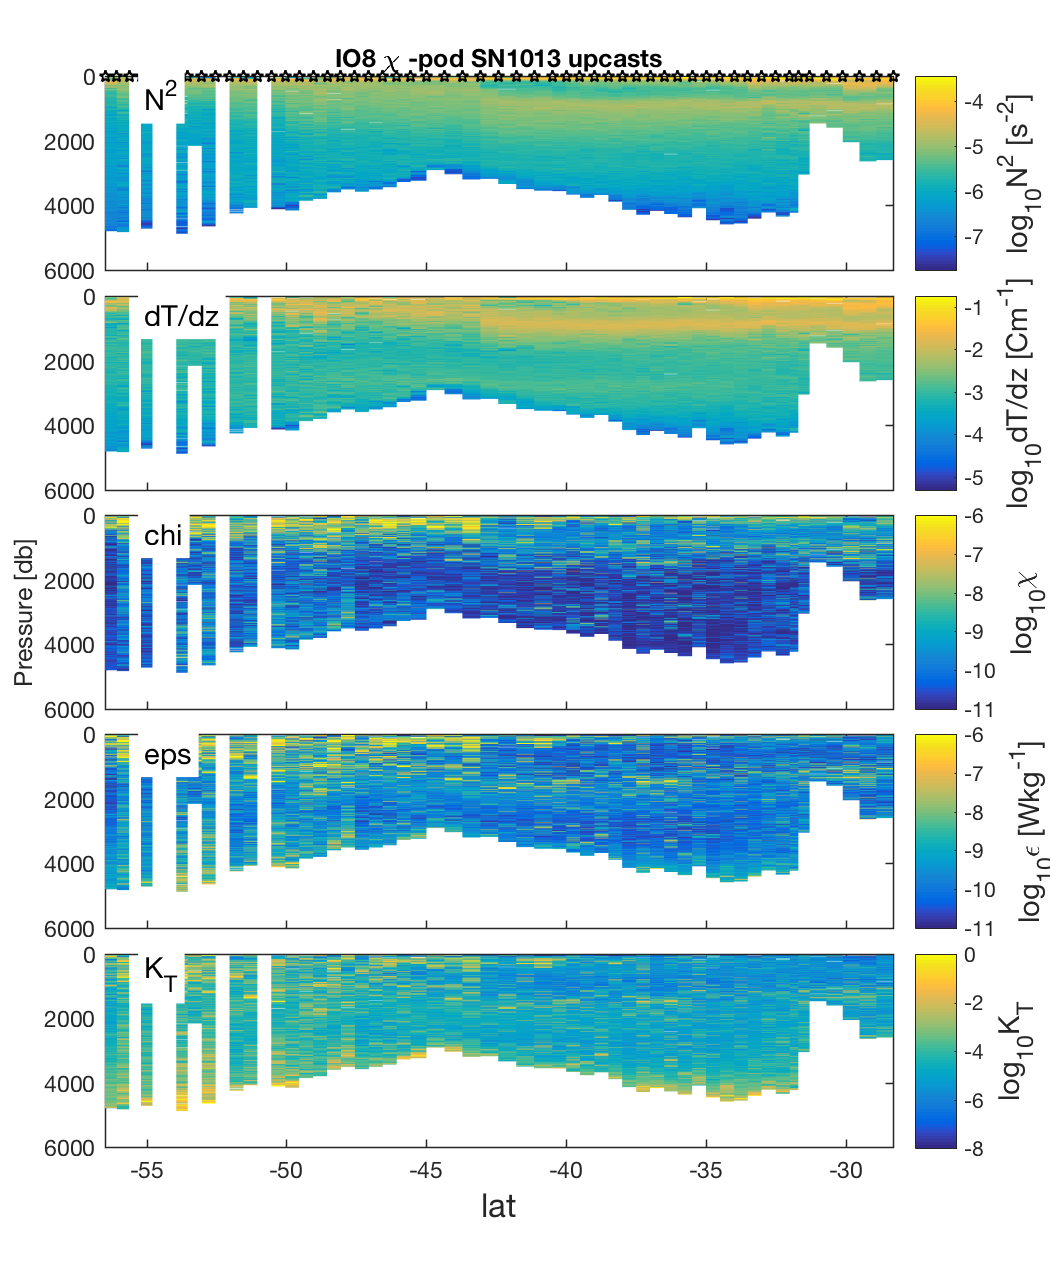
\includegraphics[scale=0.7]{XC_SN1013_Vs_lat_upAllVars.png} 
\caption{All chipod profiles from sensor SN1013. Variables are: N2, dTdz, chi, eps, and KT.} 
\label{} 
\end{figure} 

\begin{figure}[htbp] 
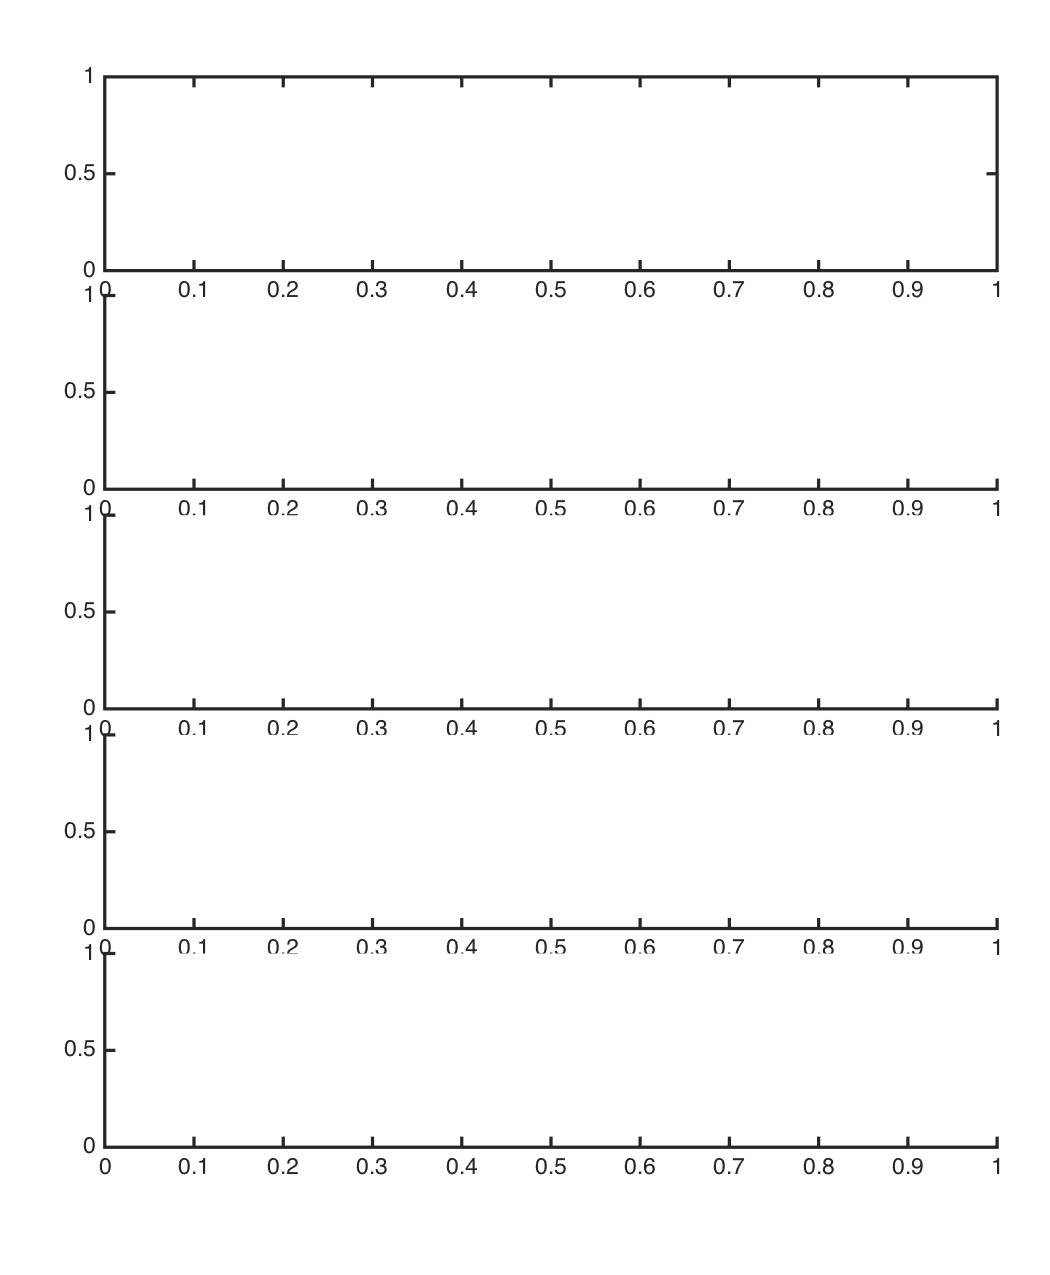
\includegraphics[scale=0.7]{XC_SN2020_Vs_lat_upAllVars.png} 
\caption{All chipod profiles from sensor SN2020. Variables are: N2, dTdz, chi, eps, and KT.} 
\label{} 
\end{figure} 

\begin{figure}[htbp] 
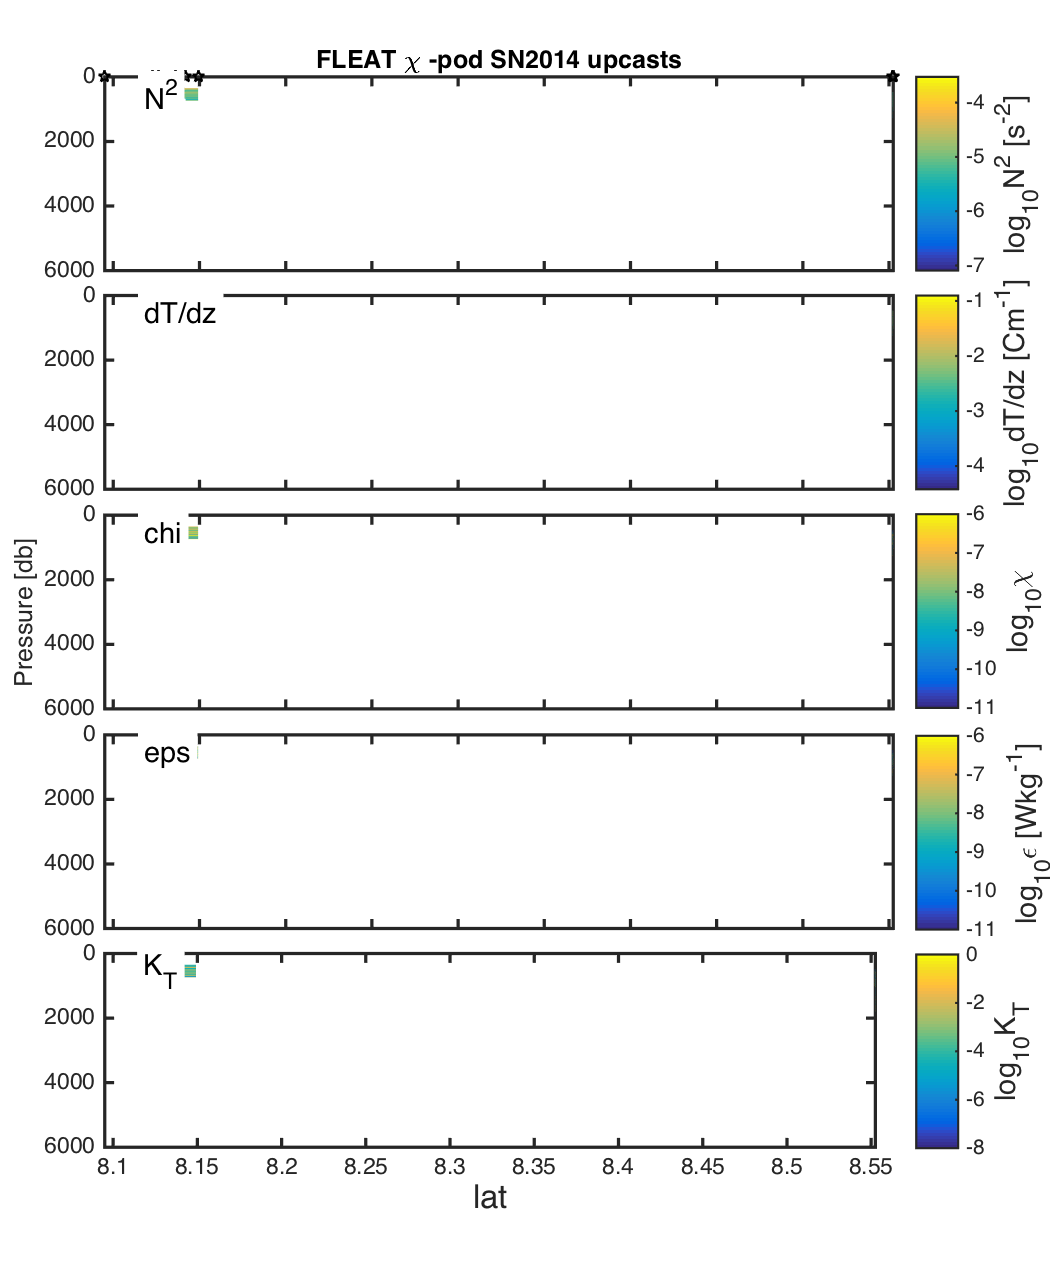
\includegraphics[scale=0.7]{XC_SN2014_Vs_lat_upAllVars.png} 
\caption{All chipod profiles from sensor SN2014. Variables are: N2, dTdz, chi, eps, and KT.} 
\label{} 
\end{figure} 

\begin{figure}[htbp] 
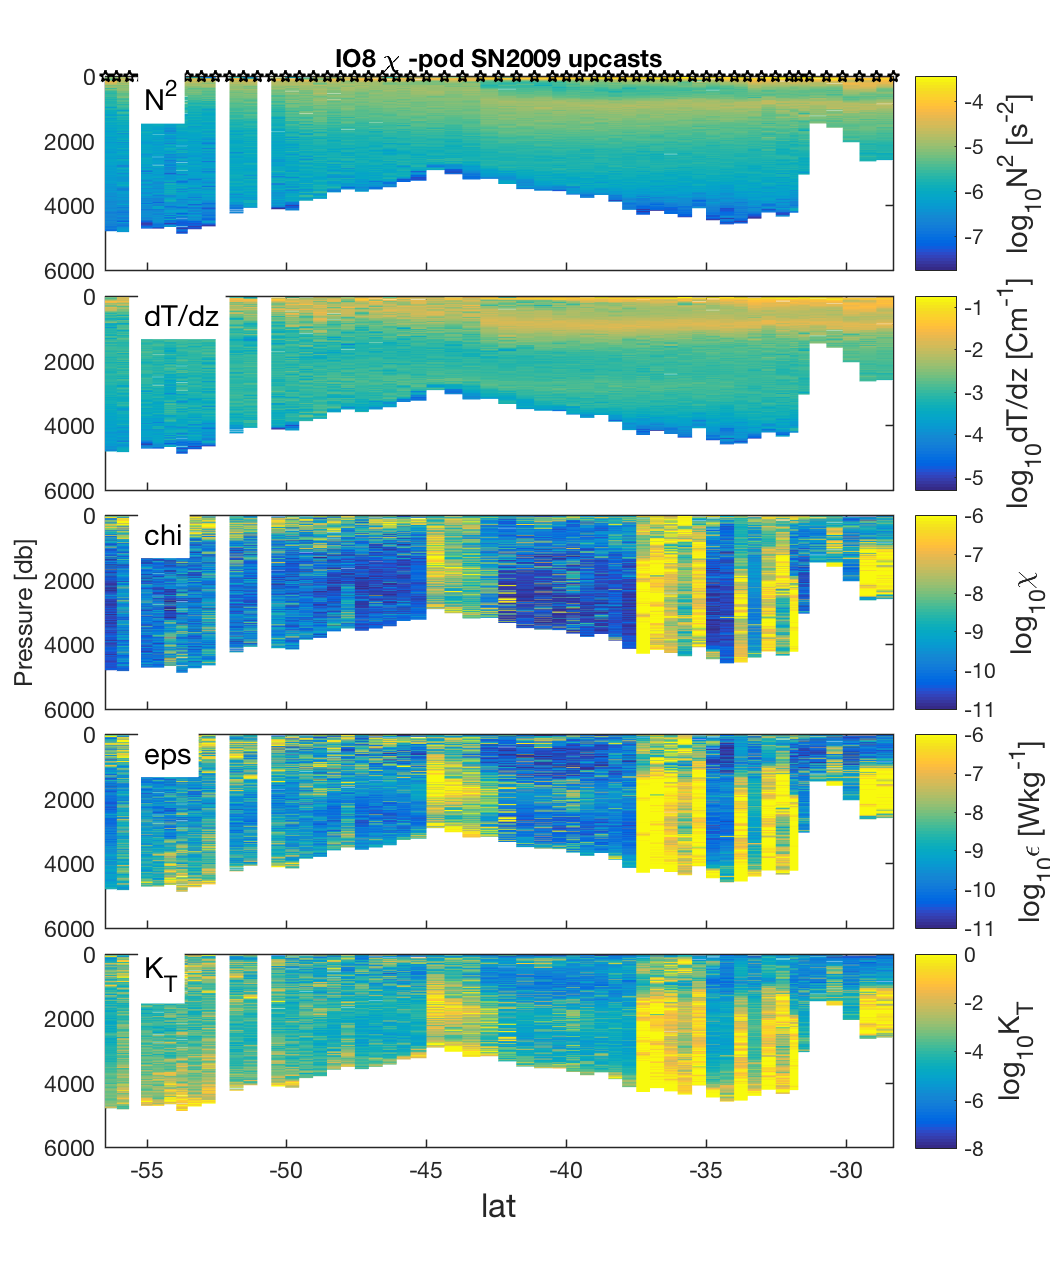
\includegraphics[scale=0.7]{XC_SN2009_Vs_lat_upAllVars.png} 
\caption{All chipod profiles from sensor SN2009. Variables are: N2, dTdz, chi, eps, and KT.} 
\label{} 
\end{figure} 

\begin{figure}[htbp] 
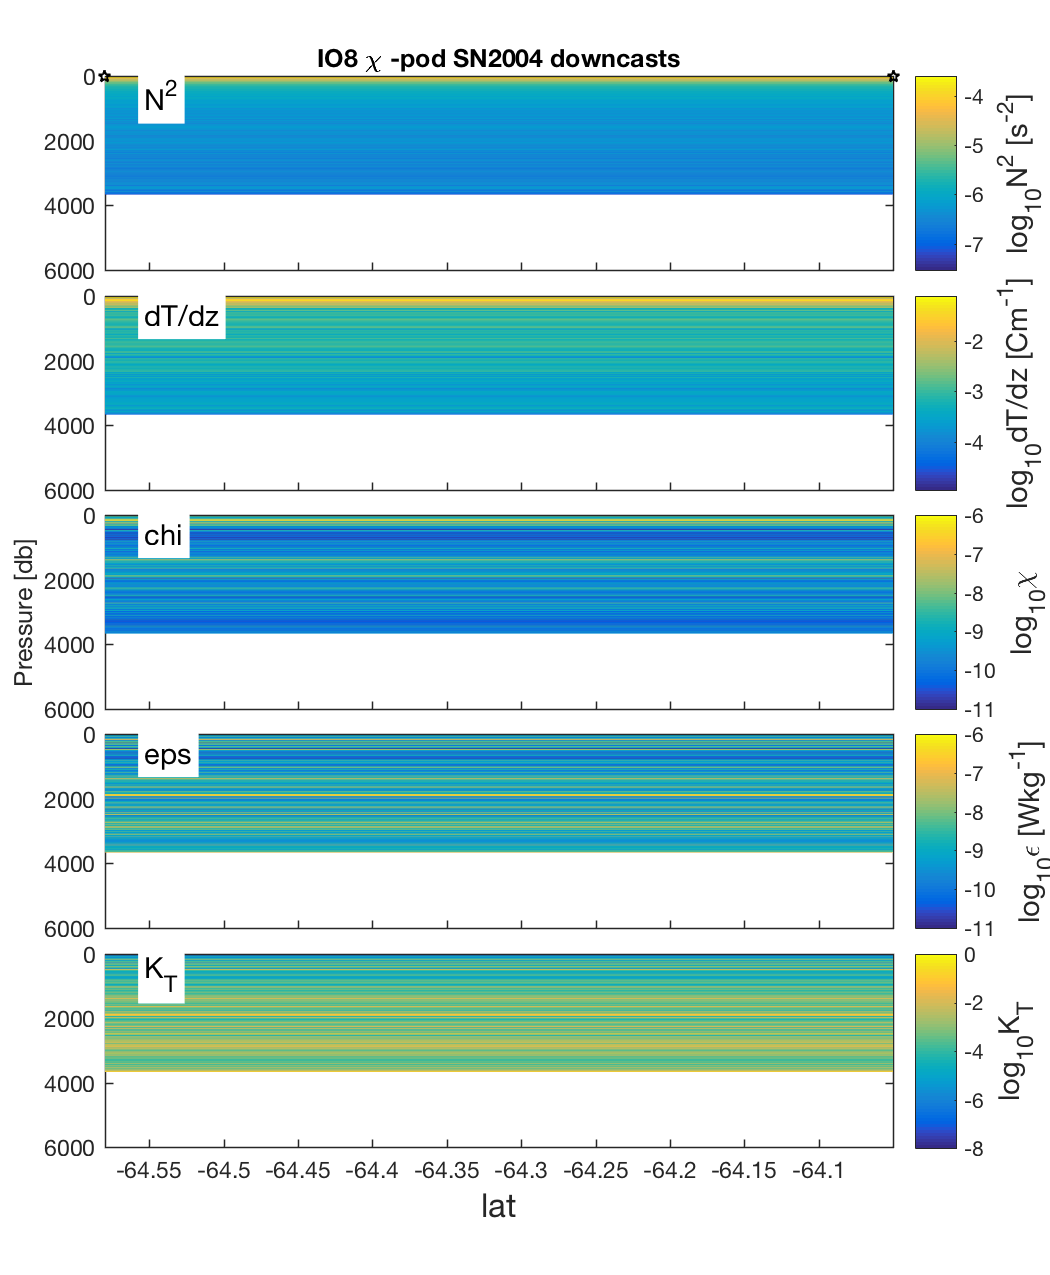
\includegraphics[scale=0.7]{XC_SN2004_Vs_lat_downAllVars.png} 
\caption{All chipod profiles from sensor SN2004. Variables are: N2, dTdz, chi, eps, and KT.} 
\label{} 
\end{figure} 

\begin{figure}[htbp] 
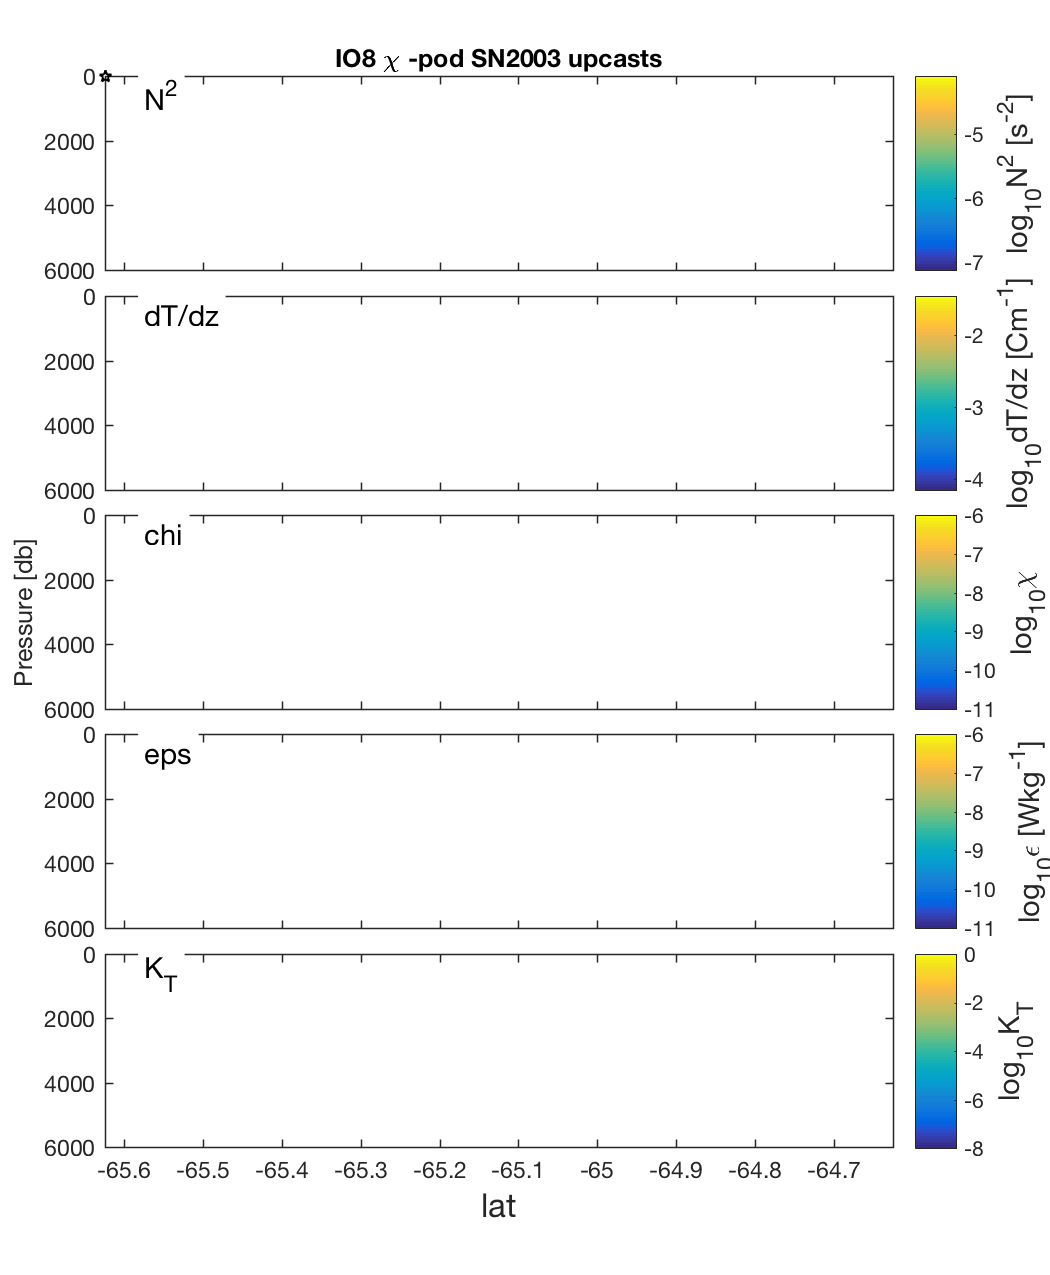
\includegraphics[scale=0.7]{XC_SN2003_Vs_lat_upAllVars.png} 
\caption{All chipod profiles from sensor SN2003. Variables are: N2, dTdz, chi, eps, and KT.} 
\label{} 
\end{figure} 

\begin{figure}[htbp] 
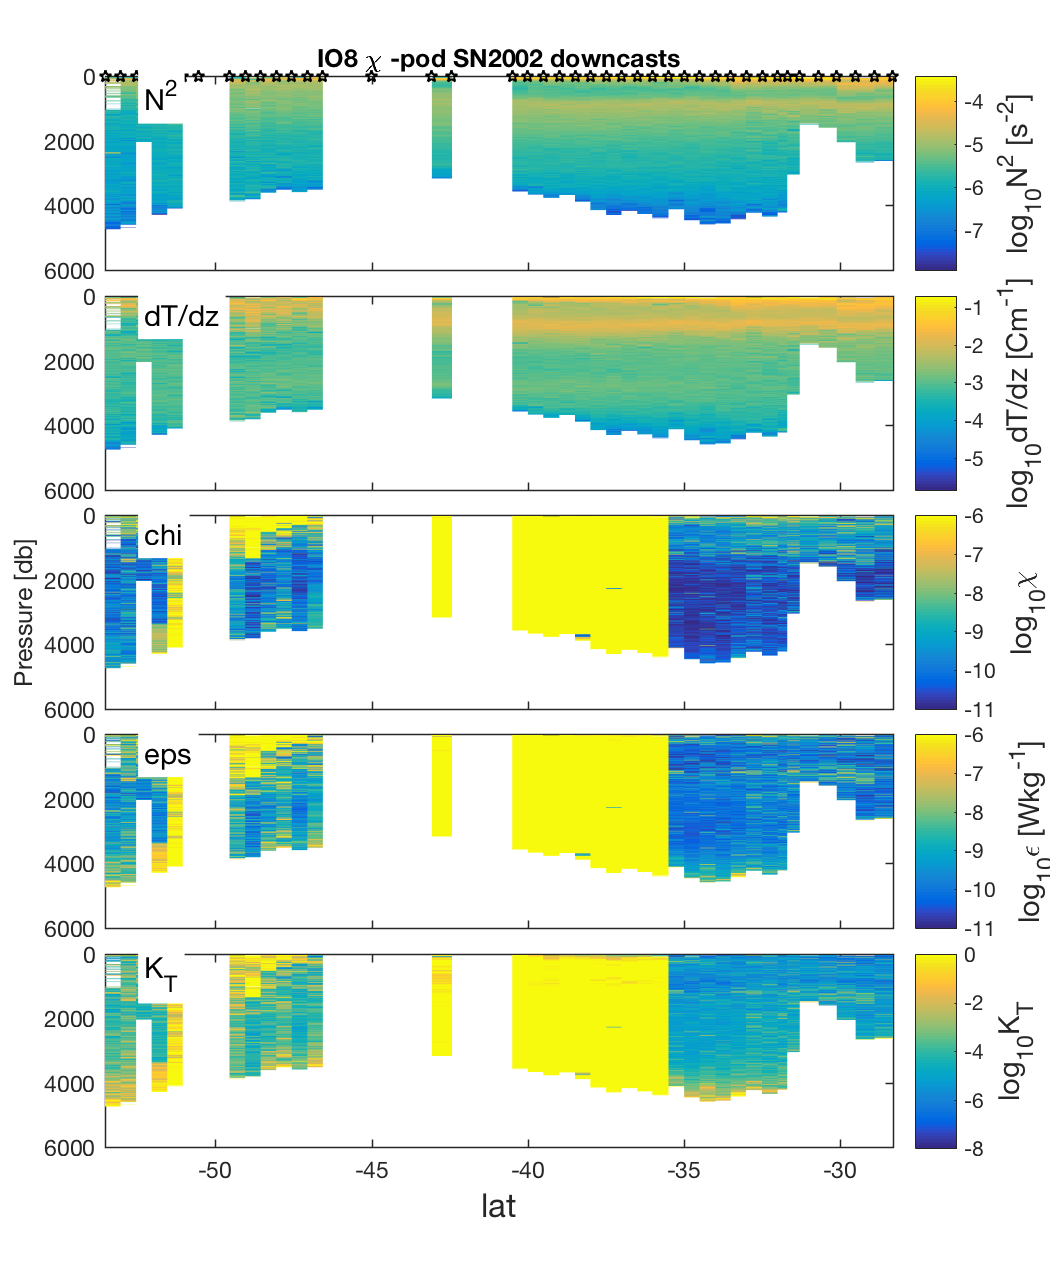
\includegraphics[scale=0.7]{XC_SN2002_Vs_lat_downAllVars.png} 
\caption{All chipod profiles from sensor SN2002. Variables are: N2, dTdz, chi, eps, and KT.} 
\label{} 
\end{figure} 

\begin{figure}[htbp] 
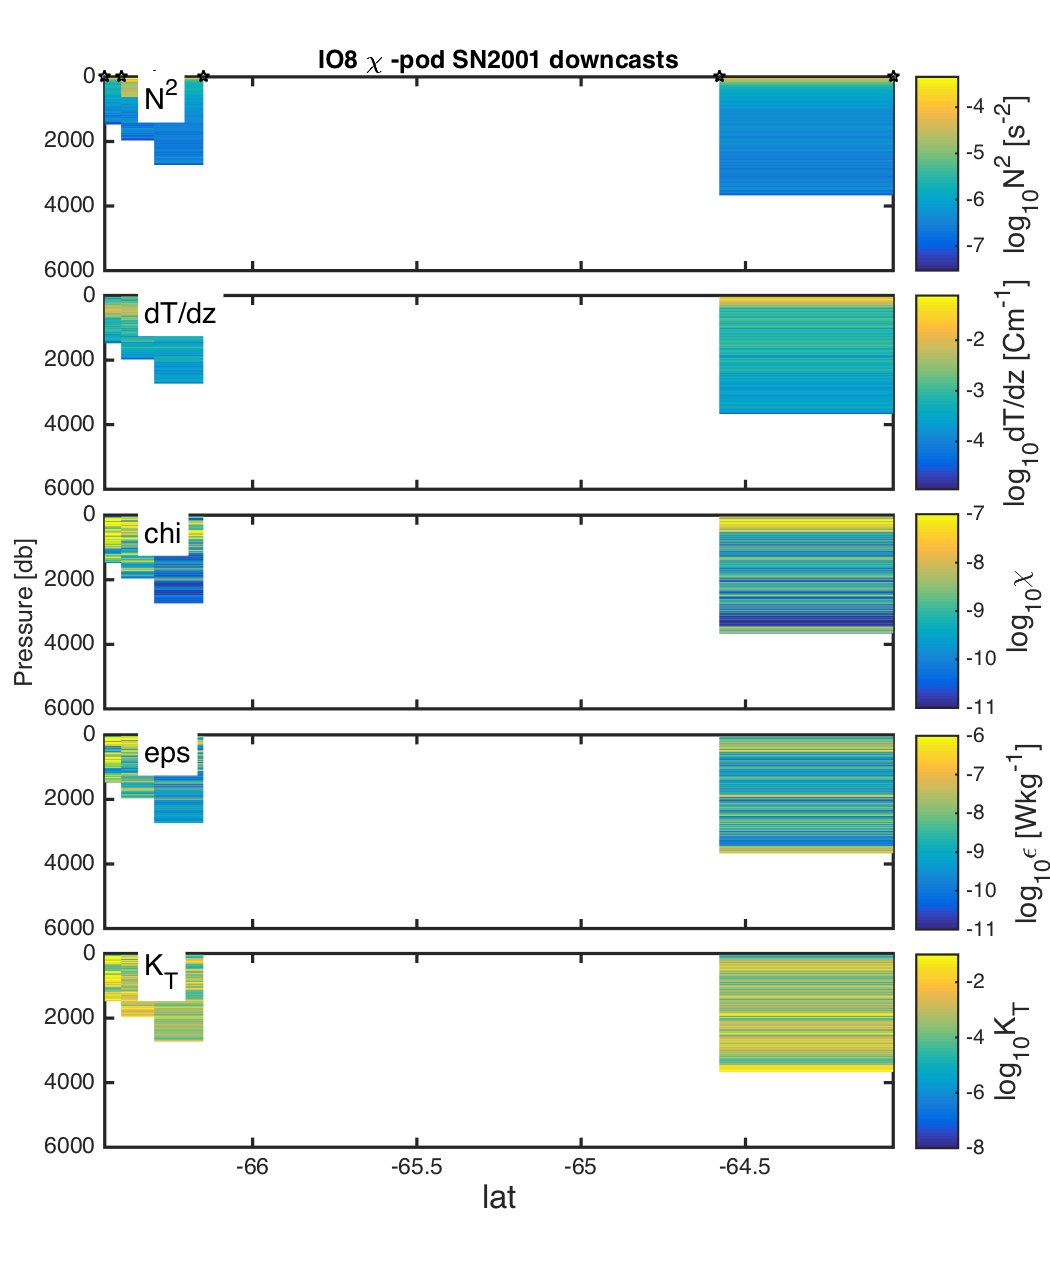
\includegraphics[scale=0.7]{XC_SN2001_Vs_lat_downAllVars.png} 
\caption{All chipod profiles from sensor SN2001. Variables are: N2, dTdz, chi, eps, and KT.} 
\label{} 
\end{figure} 

\clearpage 
\newpage 
$s\subsubsection{One variable from all Chipods} 

\begin{figure}[htbp] 
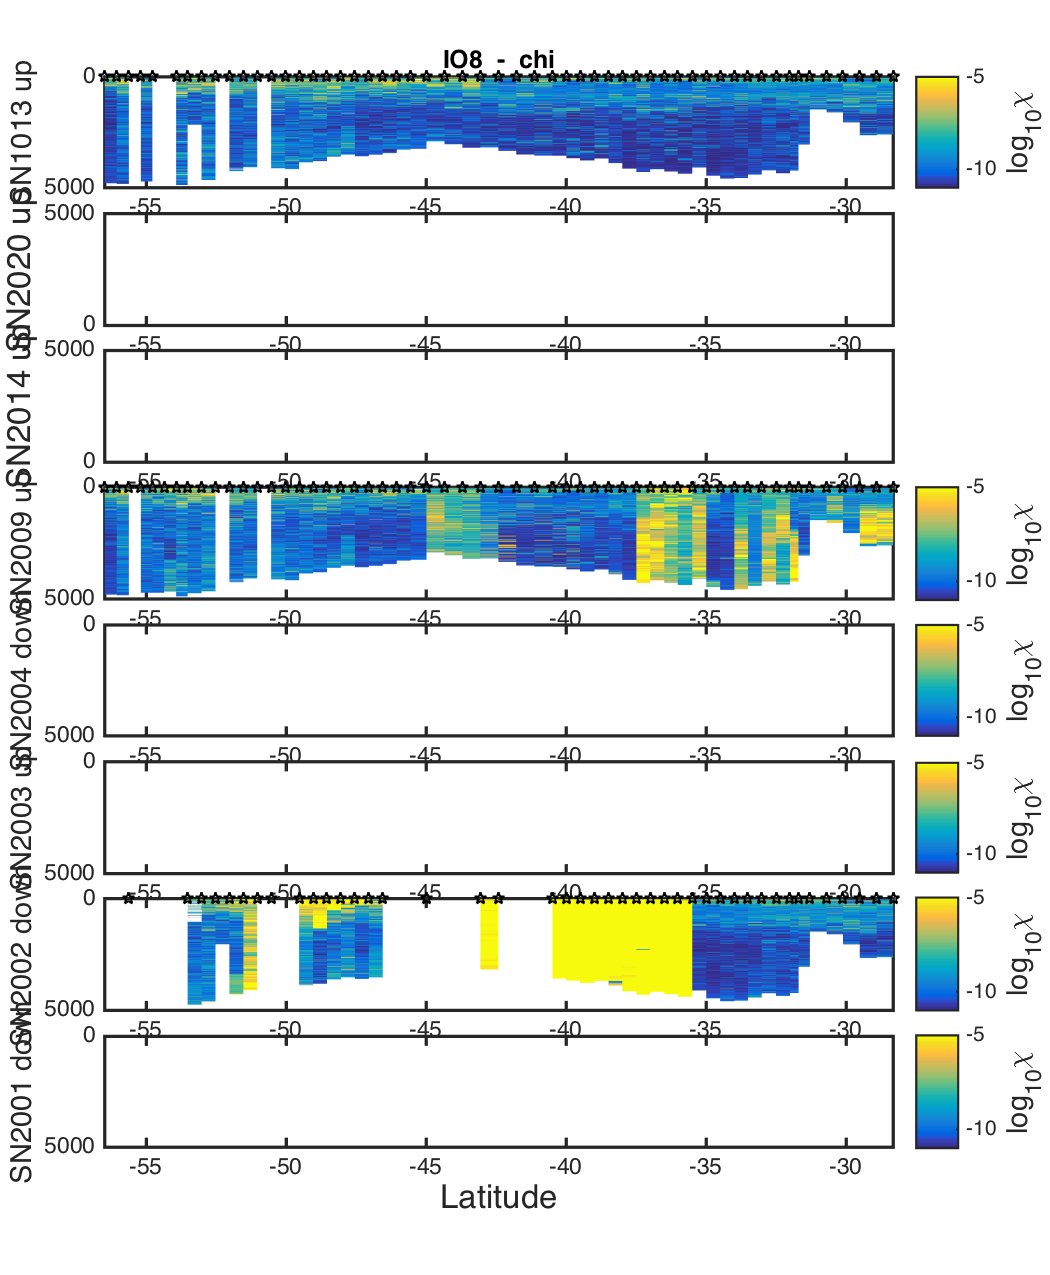
\includegraphics[scale=0.7]{IO8_chi_AllSNs_Vslat.png} 
\caption{Plot of one variable from all chipods.} 
\label{} 
\end{figure} 

\begin{figure}[htbp] 
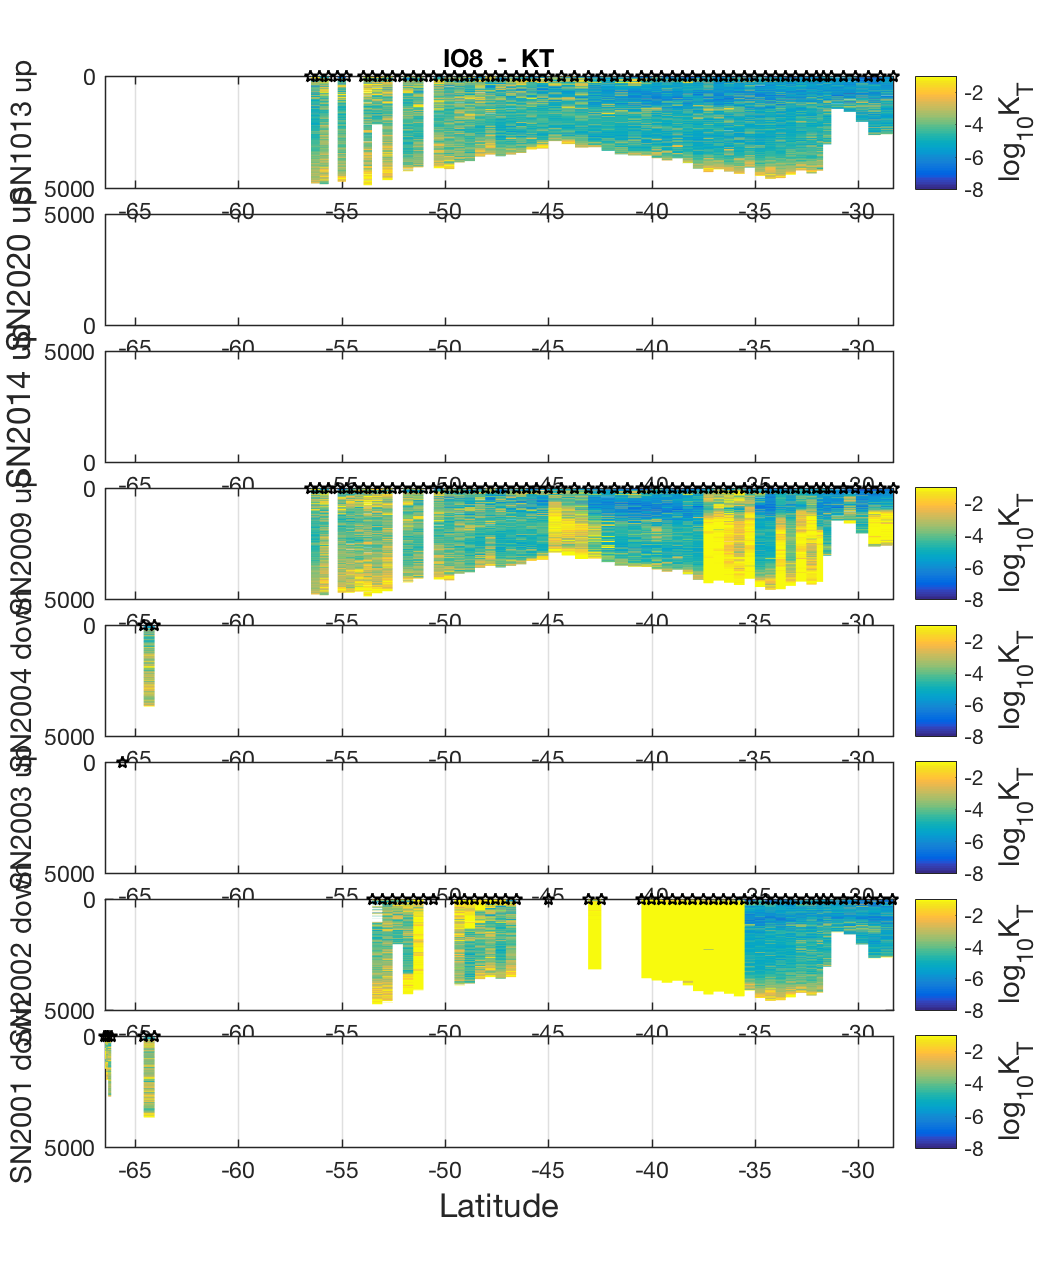
\includegraphics[scale=0.7]{IO8_KT_AllSNs_Vslat.png} 
\caption{Plot of one variable from all chipods.} 
\label{} 
\end{figure} 

\end{document}  
